\documentclass[10pt]{report}
\usepackage{/Users/bradenhoagland/latex/math}

\lhead{Braden Hoagland}
\chead{Abstract Algebra}
\rhead{}

\begin{document}
\tableofcontents

%+-------------------+
%| +---------------+ |
%| |    Chapter    | |
%| +---------------+ |
%+-------------------+
% Groups and Subgroups

\chapter{Groups and Subgroups}

%%%%%%%%%%%%%%%%%%%%
% Isomorphic Binary Structures
%%%%%%%%%%%%%%%%%%%%

\section{Isomorphic Binary Structures}

\begin{defn}{Binary Algebraic Structure}{}
	A \textbf{binary algebraic structure} $(S, *)$ is a set $S$ closed under binary operation $* : S \times S \to S$.
\end{defn}

\begin{defn}{Homomorphism}{}
	Let $(A, \cdot)$ and $(B,*)$ be binary algebraic structures. A map $\phi:A \to B$ is a \textbf{homomorphism} if
	\[
		\phi(a_1 \cdot a_2) = \phi(a_1) * \phi(a_2)
	\] for all $a_1, a_2 \in A$.
\end{defn}

\begin{defn}{Isomorphism}{}
Let $(A, \cdot)$ and $(B,*)$ be binary algebraic structures. A map $\phi:A \leftrightarrow B$ is an \textbf{isomorphism} if it is a bijective homomorphism.

If an isomorphism exists between $A$ and $B$, we write $A \simeq B$.
\end{defn}

Showing that two binary structures are isomorphic is straightforward. Find a map that is bijective and that satisfies the homomorphism property.

Showing that two binary structures are \textit{not} isomorphic is harder, as we have to show that no possible map exists. Alternatively, we can show that two binary structures have different structural properties (e.g. cardinality, commutativity), as an isomorphism preserves these properties.

\begin{prop}
	If a binary structure $(S, \cdot)$ has an identity element, it is unique.
\end{prop}
\begin{proof}
	Suppose $e_1$ and $e_2$ are both identity elements of $(S, \cdot)$. Then since $e_1$ is an identity element, $e_1 \cdot e_2 = e_2$. But since $e_2$ is an identity element, $e_1 \cdot e_2 = e_1$. Combining these two statements gives $e_1=e_2$.
\end{proof}

\begin{prop}
	Let $(A, \cdot)$ and $(B, *)$ be binary algebraic structures, and let $e$ be an identity element of $ (A, \cdot)$. If $\phi: A \leftrightarrow B$ is an isomorphism, then $\phi(e)$ is an identity element of $(B, *)$.
\end{prop}
\begin{proof}
	Let $b \in B$ be arbitrary. Then since $\phi$ is surjective and satisfies the homomorphism property, for some $a \in A$, we have
	\begin{align*}
		\phi(e) * b &= \phi(e) * \phi(a) \\
			    &= \phi(e \cdot a) \\
			    &= \phi(a) \\
			    &= b.
	\end{align*}
	Similarly, $b * \phi(e) = b$ as well, so $\phi(e)$ is an identity element of $(B, *)$.
\end{proof}

%%%%%%%%%%%%%%%%%%%%
% Groups
%%%%%%%%%%%%%%%%%%%%

\section{Groups}


\begin{defn}{Group}{}
A \textbf{group} is a binary algebraic structure $(G, \cdot)$ such that
\begin{enumerate}
	\item $(x\cdot y) \cdot z = x \cdot (y \cdot z)$ for all $x,y,z \in G$ (associativity);
	\item there is an $e \in G$ such that $e \cdot x = x \cdot e = x$ for all $x \in G$ (identity element); and
	\item for all $x \in G$, there is some $x^{-1} \in G$ such that $x^{-1} \cdot x = x \cdot x^{-1} = e$ (inverse).
\end{enumerate}
\end{defn}

\begin{note}{Group operation notation}{}
In order to clean up the notation, I'll use $xy \doteq x \cdot y$ for groups.
\end{note}

\begin{prop}
	The left and right cancellation laws hold for groups.
\end{prop}
\begin{proof}
	We'll show the left cancellation law, as the right cancellation law is similar. Let $G$ be a group, and suppose $a,b,c \in G$ and $ab = ac$, then we have
\begin{align*}
	a^{-1} (ab) &= a^{-1} (ac) \\
	(a^{-1} a) b &= (a^{-1} a) c \\
	e b &= e c \\
	b &= c.
\end{align*}
\end{proof}

Note that the proof of the left cancellation law uses left inverses and left identities, and the proof of the right cancellation law would use right inverses and right identities.

\begin{prop}
	Groups have unique solutions to linear equations.
\end{prop}
\begin{proof}
	Let $G$ be a group and let $a,b \in G$. We'll show that $ax=b$ and $ya=b$ (for variable $x$ and $y$) have unique solutions in $G$. If we let $x = a^{-1}b$, then we get
	\[
		a (a^{-1}b) = (a a^{-1})b = b,
	\] so it is a solution to the first equation. Similarly, $b a^{-1}$ is a solution of the second equation.

	Now we show that these solutions are unique. Suppose $x_1$ and $x_2$ are both solutions to $ax=b$, then we have
	\[
	ax_1 = b = ax_2,
	\] so by the cancellation law, $x_1=x_2$. The proof is similar for the equation $ya=b$.
\end{proof}

\begin{prop}
	Groups have unique identities and inverses.
\end{prop}
\begin{proof}
	First we show that the identities are unique. Suppose $e_1$ and $e_2$ are identities of a gorup $G$. Fix $x \in G$, then $e_1 x = x = e_2 x$, so by the cancellation law, $e_1=e_2$.

	Now we show that the inverses are unique. Suppose $x_1^{-1}$ and $x_2^{-1}$ are inverses of some $x \in G$. Then $x_1^{-1}x=e=x_2^{-1}x$, so by the cancellation law again, $x_1^{-1}=x_2^{-1}$.
\end{proof}

\begin{note}{}{}
	The definition of a group could very well have used just left or just right identities and inverses instead of symmetric ones. We show this with the next proposition.
\end{note}

\begin{prop}
	A group defined with left inverses and identities is the same as the earlier definition of a group.
\end{prop}
\begin{proof}
	Let $G$ be a group with left inverses and a left identity.

	First we'll show that a left inverse is a right inverse. Let $x \in G$, then there is a left inverse $x^{-1}$. Then since we have left identities,
	\[
		x x^{-1} = x (e x^{-1}) = x ( (x^{-1} x) x^{-1}) = (x x^{-1}) (x x^{-1}).
	\] 
	The earlier proof of the \textit{left} cancellation law only required the use of left identities and inverses, so we can use it here to get $x x^{-1} = e.$ Thus left inverses are also right inverses.

	Now we can show that the left identity is also a right identity. Let $x \in G$, then since we just showed that left inverses are right inverses, we have
	\[
		x e = x (x^{-1} x) = (x x^{-1}) x = e x = x.
	\] Thus the left identity is also a right identity.
\end{proof}

Note that we could have also defined a group with just \textit{right} inverses and identities. We could follow the same proof strategy as above to show that that would also be the same as our original definition of a group.

\begin{note}{}{}
A finite group can be expressed with a table. In order to satisfy the group axioms, each row and column must have exactly 1 of each group element. Tables of size 1x1, 2x2, and 3x3 can only be filled out in one way, so there is only 1 group of size 1, 1 group of size 2, and 1 group of size 3 (up to isomorphism).
\end{note}

\begin{defn}{Order}{}
The \textbf{order} of a group $G$ is its number of elements $|G|$.
\end{defn}


%%%%%%%%%%%%%%%%%%%%
% Subgroups
%%%%%%%%%%%%%%%%%%%%

\section{Subgroups}

\begin{defn}{Subgroup}{}
Let $G$ be a group, and suppose $H \subset G$. If $H$ with the induced operation from $G$ is itself a group, then $H$ is a \textbf{subgroup} of $G$.

We denote this by $H \leq G$ (improper subset) or $H < G$ (proper subset).
\end{defn}

\begin{ex}{Subgroups}{}
\begin{itemize}
	\item Subgroup: $(\mathbb{Z}, +) < (\mathbb{R},+)$.
	\item Not a subgroup: $(\mathbb{Z}, \cdot)$ vs. $(\mathbb{R}, +)$. Although $\mathbb{Z} \subset \mathbb{R}$, the operations are not the same.
\end{itemize}
\end{ex}

Subgroup diagrams can be used to visualize the subgroups of a group. Below is the subgroup diagram for $(\mathbb{Z}_4, +)$, whose subgroups are $(\{0,2\}, +)$ and $(\{0\}, +)$ (none of the other subsets of $\{0,1,2,3\}$ are closed under addition).
\begin{figure}[H]
	\centering
	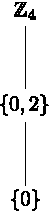
\includegraphics[scale=1]{fig/subgroup-ex.pdf}
	\caption{The subgroup diagram for $(\mathbb{Z}_4, +)$.}
\end{figure}

\begin{prop}
	\label{prop:subgroup}
	$H \subset G$ is a subgroup of $G$ if and only if
	\begin{enumerate}
		\item $H$ is closed under the binary operation of $G$;
		\item the identity element $e$ of $G$ is in $H$; and
		\item for all $x \in H$, $x^{-1} \in H$ as well.
	\end{enumerate}
\end{prop}
\begin{proof}
	The forward implication follows immediately from the definition of a subgroup, so we only show the backward implication. Conditions $(2)$ and $(3)$ show show $H$ has an identity element and inverses. Since $H \subset G$, we can view any expression in $H$ as an expression in $G$, so associativity holds. Then since $H$ is closed under the induced binary operation, it is a group. Now $H$ is a group that is also a subset of $G$, so it it is a subgroup of $G$.
\end{proof}

%%%%%%%%%%%%%%%%%%%%
% Cyclic Groups
%%%%%%%%%%%%%%%%%%%%

\section{Cyclic Groups}

Suppose $G$ is a group and $g \in G$. If we want to make a subgroup of $G$ that contains $g$, then it needs to have $g$, $g^n$ for all $n \in \mathbb{N}$, the inverses $g^{-n}$ for $n \in \mathbb{N}$, and the identity $g^0 = e$. This is formalized below.

\begin{defn}{Cyclic}{}
	Let $G$ be a group, and let $g \in G$. The set $\left\{ g^n \;|\; n \in \mathbb{Z} \right\}$ is a \textbf{cyclic} subgroup of $G$ generated by $g$ and is denoted by $\left\langle g \right\rangle$.

	If $G = \left\langle g \right\rangle$ for some $g$, then $G$ is a cyclic group.
\end{defn}

\begin{thrm}{}{}
Let $G$ be a group with $g \in G$. Then $H=\left\langle g \right\rangle$ is the smallest subgroup of $G$ that contains $g$.
\end{thrm}
\begin{proof}
	$H$ is clearly closed under the binary operation of $G$, the identity element $e=g^0$ of $G$ is in $H$, and each element of $H$ has an inverse in $H$, so by Proposition \ref{prop:subgroup}, $H$ is a subgroup of $G$.

	Removing any element from $H$ breaks at least 1 of the 3 previous conditions, so $H$ is the smallest subgroup containing $g$.
\end{proof}

\begin{note}{}{}
Since $\left\langle g \right\rangle$ is the smallest subgroup of $G$ containing $g$, any subgroup containing $g$ also contains $\left\langle g \right\rangle$.
\end{note}

\begin{prop}
	Any cyclic group is abelian.
\end{prop}
\begin{proof}
	Let $a,b \in \left\langle g \right\rangle$, then there exist $n,m \in \mathbb{Z}$ such that $g^n=a$ and $g^m=b$. Then
	\[
	ab = g^n g^m = g^{n+m}=g^{m+n}=g^m g^n=ba.
	\] 
\end{proof}

\begin{thrm}{Division Algorithm for $\mathbb{Z}$}{}
If $n$ is any integer and $m$ is a positive integer, then there exist unique integers $q$ and $r$ such that
\[
n = mq + r,
\] where $0 \leq r < m.$
\end{thrm}
\begin{proof}
	{\color{red}Do this.}
\end{proof}

\begin{prop}
	A subgroup of a cyclic group is cyclic.
\end{prop}
\begin{proof}
	Let $G = \left\langle g \right\rangle$ and let $H \leq G$. If $H = \left\{ e \right\}$, then it is clearly cyclic since $\left\langle e \right\rangle = \left\{ e \right\}$. If $H \neq \left\{ e \right\}$, then $g^{m}\in H$ for some $m \in \mathbb{Z}^+$. Consider the smallest such $m$, then we claim that $g^m$ generates $H$.

	Let $h \in H$, then since $h$ is also in $G = \left\langle g \right\rangle$, $h = g^n$ for some $n$. By the division algorithm, there are unique $q$ and $r$ such that
	\[
	n = mq+r,
\] where $0 \leq r < m$. Then $g^n = g^{nq+r}= (g^m)^q g^r$, so $g^r = (g^m)^{-q}g^n$, which is in $H$ since $g^m, g^n \in H$ and $H$ is closed. Since $m$ was the smallest positive integer such that $g^m \in H$, this implies that $r=0$. Then $n=mq$, so $g^n = (g^m)^q$. This was for arbitrary $h$, so each $h \in H$ is a power of $g^m$. jThus $H = \left\langle g^m \right\rangle$.
\end{proof}

{\color{red}Something about how subgroups of $\mathbb{Z}$ are $n\mathbb{Z}$. Also something about how group that gcd is based off of is cyclic.}

\begin{defn}{GCD}{}
Let $r$ and $s$ be positive integers. The positive generator $d$ of the cyclic group
\[
\left\{ nr+ms \;|\; n,m \in \mathbb{Z} \right\}
\] under addition is the \textbf{greatest common divisor} of $r$ and $s$. We denote it by $d = \gcd(r,s)$.
\end{defn}

\begin{defn}{Relatively prime}{}
	Positive integers $n$ and $m$ are \textbf{relatively prime} if $\gcd(n,m)=1$.
\end{defn}

\begin{prop}
	If $r$ and $s$ are relatively prime and $r \;|\; sm$, then $r \;|\; m$.
\end{prop}
\begin{proof}
	Since $r$ and $s$ are relatively prime, $ar+bs=1$ for some $a,b \in \mathbb{Z}$. Multiplying by $m$ yields
	\[
	arm + bsm = m.
	\] Now $r$ clearly divides $arm$, and $r$ divides $bsm$ since we are given $r \;|\; sm$. Thus $r$ divides $arm+bsm=m$.
\end{proof}

\begin{thrm}{}{}
	Let $G = \left\langle g \right\rangle$. If $|G| = \infty$, then $G \simeq (\mathbb{Z}, +)$. If $|G| = n$, then $G \simeq (\mathbb{Z}/n\mathbb{Z}, +)$, where $+$ here denotes addition modulo $n$.
\end{thrm}
\begin{proof}
	\textbf{Infinite order:} For all positive integers $m$, we know $g^m \neq e$ (otherwise $G$ would be finite). We claim that each $g^m$ is distinct. Suppose we have $h \neq k$ and $g^h = g^k$, and suppose without loss of generality that $h > k$. Then $g^{h-k}=e$, which is a contradiction, so $g^h \neq g^k$. Thus every element of $G$ can be written as $g^m$ for some unique $m \in \mathbb{Z}$.

	Then the map $\phi: G \leftrightarrow \mathbb{Z}$ given by $\phi(g^m) = m$ is well-defined and bijective. Additionally, we have
	\[
		\phi(g^hg^k) = \phi(g^{h+k}) = h+k = \phi(g^h) + \phi(g^k),
	\] so $\phi$ is an isomorphism between $(G, \cdot)$ and $(\mathbb{Z}, +)$.

	\textbf{Finite order:} Let $s \in \mathbb{Z}$, then by the division algorithm, $s = nq+r$, where $0 \leq r < n$. Then $g^{s}=(g^n)^q g^r = e^q g^r = g^r$. Thus each element of $G$ is in $\left\{ g^0=e, \dots, g^{n-1} \right\}$.

	We now show that each $g^i$ is unique. If $0 < k < h< n$ and $g^h=g^k$, then $g^{h-k}=e$, but this is a contradiction since $0 <h-k < n$ and $n$ is the the order of $G$. Thus $g^h \neq g^k$ when $h \neq k$, i.e. each $g^i$ is distinct. That means $\left\{ g^0=e, \dots, g^{n-1} \right\}$ has size $n$, so it comprises all of $G$.

	Then the map $\phi: G \leftrightarrow \mathbb{Z}/n\mathbb{Z}$ given by $\phi(g^m)=m$ is well-defined and bijective. Additionally, we have
	\[
		\phi(g^h g^k) = \phi(g^{h+k}) = h+k \mod n = \phi(g^h) + \phi(g^k) \mod n,
	\] so $\phi$ is an isomorphism between $(G, \cdot)$ and $(\mathbb{Z}/n\mathbb{Z}, +)$.
\end{proof}

\begin{thrm}{}{}
	Let $G= \left\langle g \right\rangle$ have order $n$, and let $h \in G$ with $h = g^m$. Then $H = \left\langle h \right\rangle$ is a cyclic subgroup of $G$ order $n/d$, where $d = \gcd(n,m)$.
\end{thrm}
\begin{proof}
	{\color{red}Do this.}
\end{proof}

\begin{cor}
	If $g$ generates $G$ and $|G|=n$, then the other generators of $G$ are of the form $g^r$, where $r$ is relatively prime to $n$.
\end{cor}
\begin{proof}
	If $d = \gcd(r,n)=1$, then $|\left\langle g^r \right\rangle| = n/d = n$, so $\left\langle g^r \right\rangle=G$. Conversely, if $d \neq 1$, then $|\left\langle g^r \right\rangle| = n/d < n$, so $\left\langle g^r \right\rangle\neq G$.
\end{proof}

%%%%%%%%%%%%%%%%%%%%
% Generating Sets
%%%%%%%%%%%%%%%%%%%%

\section{Generating Sets}

\begin{prop}
	Let $\left\{ H_{\alpha} \right\}_{\alpha \in \mathcal{J}}$ be subgroups of $G$, then $\bigcap_{\alpha}H_{\alpha}$ is also a subgroup of $G$.
\end{prop}
\begin{proof}
	\textbf{Closure:} Let $a,b \in \bigcap_{\alpha}H_{\alpha}$, then $a,b \in H_{\alpha}$ for all $\alpha$. Since each $H_{\alpha}$ is a group, $ab \in H_{\alpha}$ for all $\alpha$. Thus $ab \in \bigcap_{\alpha}H_{\alpha}$.

	\textbf{Associativity:} Each $H_{\alpha}$ is associative, so elements in their intersection must also be associative.

	\textbf{Identity:} Since each $H_{\alpha}$ is a group, $e \in H_{\alpha}$ for all $\alpha$, so $e \in \bigcap_{\alpha}H_{\alpha}$.

	\textbf{Inverses:} Fix $a \in \bigcap_{\alpha}H_{\alpha}$, then $a \in H_{\alpha}$ for all $\alpha$. Then since each $H_{\alpha}$ is a group, $a^{-1} \in H_{\alpha}$ for all $\alpha$, so $a^{-1} \in \bigcap_{\alpha}H_{\alpha}$.
\end{proof}

Now suppose we have some set $S \doteq \left\{ g_i \;|\; i \in \mathcal{J}\right\}$ that lies in a group $G$. There is at least one subgroup of $G$ that contains each $g_i$ (e.g. $G$ itself). Then by the above proposition, we can take the intersection of all of these subgroups to get the smallest possible subgroup of $G$ containing $S$. Since we know that such a smallest subgroup exists, it makes sense to figure out what it looks like.

\begin{defn}{Subgroup of Generating Set}{}
	Let $G$ be a group, and let $g_i \in G$ for all $i \in \mathcal{J}$. The \textbf{subgroup} generated by $S \doteq \left\{ g_i \;|\; i \in \mathcal{J} \right\}$ is the smallest subgroup of $G$ containing $S$, and its \textbf{generating set} is $S$.

If  a group $G$ is generated by some finite generating set, then it is \textbf{finitely generated.} 
\end{defn}

\begin{note}{}{}
The phrase ``$g$ is a generator of $G$" could mean
\begin{enumerate}
	\item $G = \left\langle g \right\rangle$; or
	\item $g \in S$, where $G = \left\langle S \right\rangle$.
\end{enumerate}
Use context to determine which of these is meant.
\end{note}

\begin{thrm}{}{}
	Let $g_i \in G$ for all $i \in \mathcal{J}$. The subgroup $H$ of $G$ generated by $\left\{ g_i \;|\; i \in \mathcal{J} \right\}$ has as elements all finite products of integral powers of the $g_i$.
\end{thrm}
\begin{proof}
	Let $K$ denote the set of all finite products of intergral powers of the $g_i$, then clearly $K \subset H$ (since $H$ must be closed under the group operation). If we show that $K$ is a subgroup, then since $H$ is the smallest subgroup containing the $g_i$, we'll have $H \subset K$. This implies $H=K$, which is what we want.

	Thus we now show that $K$ is a subgroup. The product of elements of $K$ is clearly also in $K$, so it is closed under the group operation. The element $(g_i)^0 = e$ is in $K$, so it contains the identity element. Any $k \in K$ can be written as a sequence of products, so reverse the order of the products and negate each exponent to get the inverse $k^{-1}$, which is clearly also in $K$. Thus $K$ is a subgroup, so $H=K$.
\end{proof}

\begin{ex}{}{}
	Let $a,b \in G$ for some group $G$, then $\left\langle a,b \right\rangle$ contains all possible finite products involving $a$ and $b$. These include
	\begin{itemize}
		\item $a$,
		\item $b^7$,
		\item $a^2 b^3$, and
		\item $a b a^{-1} b^2$.
	\end{itemize}
	Note that we can't necessarily simplify that last product because $G$ might not be abelian.
\end{ex}

%+-------------------+
%| +---------------+ |
%| |    Chapter    | |
%| +---------------+ |
%+-------------------+
% Permutations, Cosets, and Direct Products

\chapter{Permutations, Cosets, and Direct Products}

%%%%%%%%%%%%%%%%%%%%
% Permutation Groups
%%%%%%%%%%%%%%%%%%%%

\section{Permutation Groups}

\begin{defn}{Permutation}{}
A \textbf{permutation} of a set $X$ is a bijective function $\phi:X \leftrightarrow X$.
\end{defn}

If $\tau$ and $\sigma$ are permutations of $X$, consider their composition $\sigma \tau$. It is easily shown that this is also a bijection from $X$ to itself, so the composition of permutations is again a permutation.

\begin{figure}[H]
	\centering
	
\includegraphics[scale=1.2]{fig/permutation-composition.pdf}
	\caption{The composition $\sigma \tau$.}
\end{figure}

\begin{note}{Permutation Notation}{}
The permutation
\[
\sigma =
\begin{pmatrix}
	1 & 2 & 3 \\
	3 & 2 & 1
\end{pmatrix}
\] maps $1 \mapsto 3$, $2 \mapsto 2$, and $3 \mapsto 1$.
\end{note}

\begin{defn}{Symmetric Group}{}
The \textbf{symmetric group} $S_n$ (of degree $n$) is the set of all permutations of $\left\{ 1, \dots, n \right\}$.

If $X$ is any set, then $S_X$ is shorthand for $S_{|X|}$.
\end{defn}

Note that if $X$ has $n$ elements, then $S_X$ has $n!$ elements.

\begin{thrm}{}{}
Let $X$ be a nonempty set, then the symmetric group $S_X$ is a group under permutation composition.
\end{thrm}
\begin{proof}
	$S_X$ is closed under permutation composition since the composition of permutations is also a permutation. It is associative because the composition of functions is associative. The permutation that maps $x \mapsto x$ for each $x \in X$ acts as the identity element. Finally, since bijections have inverses, so does each permutation. Thus $S_X$ is a group.
\end{proof}

%%%%%%%%%%%%%%%%%%%%
% Cayley's Theorem
%%%%%%%%%%%%%%%%%%%%

\section{Cayley's Theorem}

\begin{lem}
	Let $G$ and $G'$ be groups, and let $\phi:G \hookrightarrow  G'$ be a one-to-one homomorphism. Then $\phi(G)$ is a subgroup of $G'$ and $\phi$ is an isomorphism between $G$ and $\phi(G)$.
\end{lem}
\begin{proof}
	By Proposition \ref{prop:subgroup}, in order to show that $\phi(G)$ is a subgroup of $G'$, we need only show that $\phi(G)$ is closed, has an identity, and has inverses for every element.

	Let $x',y' \in \phi(G)$, then there exist $x,y\in G$ such that $\phi(x)=x'$ and $\phi(y)=y'$. Then since $\phi$ is a homomorphism, $x'y' = \phi(x)\phi(y) = \phi(xy)$, so $\phi(G)$ is closed under the group operation of $G'$.

	Let $e'$ be the identity of $G'$, then $e'\phi(e) = \phi(e) = \phi(ee) = \phi(e) \phi(e)$, so by cancellation, $e' = \phi(e)$. Thus $\phi(G)$ contains the identity element.

	Fix $x \in G$ then for $x'=\phi(x)$, we have $e'=\phi(e) = \phi(xx^{-1}) = \phi(x)\phi(x^{-1}) = x'\phi(x^{-1}).$ Then the inverse of $x'$ is $\phi(x^{-1})$, so $\phi(G)$ has inverses for each element.

	This shows that $\phi(G)$ is a subgroup of $G'$. Now $\phi$ is already one-to-one and homomorphic, and it is clearly onto $\phi(G)$, so $\phi$ is an isomorphism between $G$ and $\phi(G)$.
\end{proof}

\begin{thrm}{Cayley's Theorem}{cayley}
Every group is isomorphic to a group of permutations.
\end{thrm}
\begin{proof}
	Let $G$ be a group. We will show that $G$ is isomorphic to some subgroup of $S_{G}$. By the previous lemma, we only need to define a one-to-one homomorphism $\phi:S\hookrightarrow S_G$. Fix $x \in G$, then define $\lambda_x:G\to G$ by $\lambda_x(g) =xg$. We claim that $\lambda_x$ is a permutation of $G$.

	If $\lambda_x(a)=\lambda_x(b)$, then $xa=xb$, so by cancellation, $a=b$. Thus $\lambda_x$ is one-to-one. Fix $x \in G$, then $\lambda_x$ maps $x^{-1}g \mapsto g$, so $\lambda_x$ is onto. Thus $\lambda_x$ is a permutation of $G$.

	Now define $\phi:G\to S_G$ by $\phi(x)=\lambda_x$, then we claim that $\phi$ is an injective homomorphism. If $\phi(x)=\phi(y)$, then $\lambda_x(g)=\lambda_y(g)$ for all $g$. Then $xg=yg$, so by cancellation, $x=y$, so $\phi$ is isomorphic. Additionally, for $x,y\in G$, we have
	\[
		\lambda_{xy}(g)=(xy)g=x(yg)=(\lambda_x \circ \lambda_y)(g),
	\] so $\phi(xy)=\lambda_{xy}=\lambda_x \circ \lambda_y = \phi(x)\circ\phi(y)$. Thus $\phi$ is homomorphic.

	Then by the previous lemma, $\phi$ is an isomorphism between $G$ and $\phi(G)$ (which is a subgroup of $S_G$).
\end{proof}

\begin{defn}{Regular Representation}{}
	The map $\phi$ in the proof above is the \textbf{left regular representation} of $G$. $\phi(x)$ is the permutation of $G$ gotten by left multiplying every element of $G$ by $x$.

	The \textbf{right regular representation} is defined similarly.
\end{defn}

\begin{ex}{Regular Representation}{}
Let $G=\left\{ e,a,b \right\}$, then the table representing $G$ is
\begin{center}
	\begin{tabular}{c||c|c|c}
		& \textbf{e}  & \textbf{a}  & \textbf{b}  \\
		\hline
		\hline
		\textbf{e}  & e & a & b \\
		\hline
		\textbf{a}  & a & b & e \\
		\hline
		\textbf{b}  & b & e & a
	\end{tabular}
\end{center}
and its left regular representation has elements
\begin{gather*}
	\lambda_e =
	\begin{pmatrix}
		e & a & b \\
		e & a & b
	\end{pmatrix} \quad
	\lambda_a =
	\begin{pmatrix}
		e & a & b \\
		a & b & e
	\end{pmatrix} \\
	\lambda_b =
	\begin{pmatrix}
		e & a & b \\
		b & e & a
	\end{pmatrix}.
\end{gather*}
\end{ex}


%%%%%%%%%%%%%%%%%%%%
% Orbits and Cycles
%%%%%%%%%%%%%%%%%%%%

\section{Orbits and Cycles}

\begin{defn}{Orbit}{}
	Let $\sigma$ be a permutation of $X$. Define an equivalence relation on $X$ by saying $x \sim y$ if $y=\sigma^n(x)$ for some $n \in \mathbb{Z}$. The equivalence classes of $X$ determined by $\sim$ are the \textbf{orbits} of $X$.
\end{defn}

\begin{ex}{Orbits}{}
Consider the permutation
\[
\sigma=
\begin{pmatrix}
	1&2&3&4&5&6&7&8\\
	3&8&6&7&4&1&5&2
\end{pmatrix}.
\] It has three cycles, pictured below.
\begin{center}
\begin{tikzcd}
1 \arrow[d] &              &                        &                        &             & 4 \arrow[ld] \\
3 \arrow[r] & 6 \arrow[lu] & 2 \arrow[r, bend left] & 8 \arrow[l, bend left] & 7 \arrow[r] & 5 \arrow[u]
\end{tikzcd}

\end{center}

It has three equivalence classes: $\left\{ 1,3,6 \right\}$, $\left\{ 2, 8 \right\},$ and $\left\{ 4,5,7 \right\}$.
\end{ex}

\begin{defn}{Cycle}{}
	A finite permutation $\sigma\in S_n$ is a \textbf{cycle} if it has at most 1 orbit containg more than 1 element. The \textbf{length} of a cycle is the number of elements in its largest orbit.
\end{defn}

\begin{ex}{Cycles}{}
The permutation below is a cycle.

\begin{center}
\begin{tikzcd}
1 \arrow[r] & 2 \arrow[d] & 4 \arrow[loop, distance=2em, in=35, out=325] \\
5 \arrow[u] & 3 \arrow[l] &                                             
\end{tikzcd}
\end{center}

The next permutaiton is also a cycle.

\begin{center}
\begin{tikzcd}
1 \arrow[r] & 2 \arrow[d]  \\
            & 3 \arrow[lu]
\end{tikzcd}
\end{center}

The next permutation, however, is \textit{not} a cycle.

\begin{center}
\begin{tikzcd}
1 \arrow[r, bend left] & 2 \arrow[l, bend left] & 3 \arrow[r, bend left] & 4 \arrow[l, bend left] & 5 \arrow[loop, distance=2em, in=215, out=145]
\end{tikzcd}
\end{center}
\end{ex}

\begin{defn}{Disjoint Cycles}{}
A collection of cycles is \textbf{disjoint} if each element is moved by at most 1 of the cycles.
\end{defn}

Multiplication of disjoint cycles is clearly commutative (permutation in general is not).

\begin{thrm}{}{}
	Every permutation $\sigma$ of a finite set is a product of disjoint cycles.
\end{thrm}
\begin{proof}
	Let $B_1, \dots, B_r$ be the orbits of $\sigma$, and define the cycle $\mu_i$ by
	\[
		\mu_i(x) =
		\begin{cases}
			\sigma(x) & x \in B_i \\
			x & \text{otherwise}.
		\end{cases}
	\] 
	Clearly $\sigma = \prod_{i=1}^r \mu_i$. Since the orbits are disjoint (because they are equivalence classes), the cycles $\mu_1, \dots, \mu_r$ are as well.
\end{proof}

\begin{note}{Cyclic notation}{}
	When writing a cycle, we write the permutation with a single row (the elements of the cycle in order). For example, $(1\;2\;3)$ is the cycle that sends $1\mapsto 2$, $2\mapsto 3$, and $3\mapsto 1$.
\end{note}

\begin{defn}{Transposition}{}
A \textbf{transposition} is a cycle of length 2.
\end{defn}

\begin{ex}{Transpositions}{}
	The cycle $(1\;2)$ is a transposition, but the cycle $(1\;2\;3)$ is not.
\end{ex}

\begin{cor}
	Any permutation of a finite set of 2 or more elements is a product of transpositions.
\end{cor}
\begin{proof}
	Since
	\[
		(x_1 \cdots x_n) = (x_1\;x_n) (x_1\;x_{n-1}) \dots (x_1\;x_2),
	\] every cycle is the product of transpositions. Then since every permutation of a finite set is the product of cycles, every permutation is also the product of transpositions.
\end{proof}

\begin{ex}{}{}
	$(1\;6)(2\;5\;3) = (1\;6)(2\;3)(5\;3)$.
\end{ex}

\begin{ex}{}{}
	The identity permutation $\iota$ for $S_n$, where $n \geq 2$, can be written $(1\;2)(1\;2)$.
\end{ex}

%%%%%%%%%%%%%%%%%%%%
% Alternating Groups
%%%%%%%%%%%%%%%%%%%%

\section{Alternating Groups}

\begin{defn}{Even/Odd Permutation}{}
	A permutation of a finite set is \textbf{even} if it is the product of an even number of transpositions. It is \textbf{odd} if it is the product of an odd number of transpositions.
\end{defn}

\begin{defn}{Alternating Group}{}
The \textbf{alternating group} $A_n$ of degree $n$ is the set of even permutations in $S_n$.
\end{defn}

\begin{thrm}{}{}
No permutation in $S_n$ is both even and odd. 
\end{thrm}
\begin{proof}
	It is clear that the set $\left\{ 1,\dots, n \right\}$ is isomorphic to the rows of the identity matrix $I_n$. Then a permutation in $S_n$ corresponds to swapping rows of $I_n$. Thus if a permutation were both even and odd, the determinant of the resulting matrix would be both $1$ and $-1$, which is impossible. Thus no permutation can be both even and odd.
\end{proof}

\begin{thrm}{}{}
For $n\geq 2$, the number of even permutations in $S_n$ is equal to the number of odd permutations in $S_n$.
\end{thrm}
\begin{proof}
	Let $B_n$ denote the set of odd permutations in $S_n$. If we find a bijection between $A_n$ and $B_n$, then they must have the same number of elements, so this is what we'll do.

	Let $\tau$ be a transposition in $S_n$ (it exists since $n \geq 2$). Define a function $\lambda_{\tau}:A_n \to  B_n$ by $\lambda_{\tau}(\sigma) = \tau \sigma$. Since $\sigma \in A_n$, it is even, so $\tau \sigma$ is odd, so $\tau \sigma \in B_n$. We claim that $\lambda_{\tau}$ is a bijection.

	If $\lambda_{\tau}(\sigma) = \lambda_{\tau}(\mu)$, then $\tau \sigma = \tau \mu$, so by cancellation (since $S_n$ is a group), $\sigma = \mu$. Thus $\lambda_{\tau}$ is one-to-one. Additionally, the inverse of a transposition is itself, so if $\rho \in B_n$, then $\tau^{-1}\rho = \tau \rho \in A_n$ and $\lambda_{\tau}(\tau^{-1}\rho) = \rho$. Thus $\lambda_{\tau}$ is onto.

	We have found a bijection between $A_n$ and $B_n$, so $|A_n| = |B_n|$.
\end{proof}

\begin{thrm}{}{}
For $n\geq 2$, $A_n$ forms a subgroup of $S_n$ of order $n!/2$.
\end{thrm}
\begin{proof}
	$|S_n|=n!$, so by the previous theorem, we know $|A_n|=|B_n|=n!/2$. We now show the three criteria from Proposition \ref{prop:subgroup} in order to show that $A_n$ is a subgroup of $S_n$.

	If $\sigma$ and $\mu$ are even, then clearly so is $\sigma \mu$, so $A_n$ is closed under permutation composition.

	Since $n\geq 2$, the identity transposition $\iota$ can be written as $(1\;2)(1\;2)$, so $\iota$ is even.

	Since the inverse of a transposition is itself, decompose a permutation $\sigma$ into its transpositions, then reverse the order of the transpositions to get its inverse $\sigma^{-1}$, which is clearly also even.

	Thus by Proposition \ref{prop:subgroup}, $A_n$ is a subgroup of $S_n$.
\end{proof}


%%%%%%%%%%%%%%%%%%%%
% Cosets and Lagrange's Theorem
%%%%%%%%%%%%%%%%%%%%

\section{Cosets and Lagrange's Theorem}


\begin{thrm}{}{}
Let $H$ be a subgroup of $G$. The relation $\sim_L$ on $G$ is defined by saying $x \sim_L y$ if $x^{-1}y \in H$. The relation $\sim_R$ on $G$ is defined by saying $x \sim_R$ if $xy^{-1} \in H$. Both of these relations are equivalence relations on $G$.
\end{thrm}
\begin{proof}
	We only prove this for the relation $\sim_L$, as the proof for $\sim_R$ is similar. Since $H$ is a group, it has an identity, so $x^{-1} x = e \in H$. Thus $x \sim_L x$, i.e. the relation is reflexive. If $x \sim_L y$, then $x^{-1}y \in H$, so since $H$ is a group and has inverses, $(x^{-1}y)^{-1}=y^{-1}x\in H$. Thus $y \sim_L x$, i.e. the relation is symmetric. Finally, given $x \sim_L y$ and $y \sim_L z$, we know $x^{-1}y, y^{-1}z \in H$. Since $H$ is closed and associative, we have $x^{-1}yy^{-1}z = x^{-1}z \in H$. Thus $x \sim_L z$, i.e. the relation is transitive.
\end{proof}

Suppose we partition a group $G$ using the equivalence relation $\sim_L$, then the cell of the partition that contains $g \in G$ is of the form $\left\{ gh \;|\; h \in H \right\}$. We denote this set by $gH$. Similarly, cells based on the partition from $\sim_R$ are of the form $Hg \doteq \left\{ hg \;|\; h \in H \right\}$.

\begin{defn}{Coset}{}
Let $H$ be a subgroup of $G$. Then $gH$ is the \textbf{left coset} of $H$ in $G$ containing $g$. $Hg$ is the \textbf{right coset} of $H$ in $G$ containing $g$.
\end{defn}

\begin{prop}
	Let $H$ be a subgroup of an abelian group $G$, then the left cosets of $H$ are the same as the right cosets of $H$.
\end{prop}
\begin{proof}
	$gh=hg$ if $G$ is abelian.
\end{proof}

\begin{prop}
	Every left and right coset of $H$ has the same cardinality as $H$.
\end{prop}
\begin{proof}
	Fix $g$, then we will construct a bijective map from $H$ to $gH$. Define $\phi(h):H\to gH$ by $\phi(h)=gh$. This is clearly onto $gH$ (by the definition of left cosets). Now suppose $\phi(h_1)=\phi(h_2)$, then $gh_1=gh_2$, so by cancellation, $h_1=h_2$. Thus $\phi$ is a bijection, so $H$ and $gH$ have the same cardinality for all $g$. The case for right cosets is similar.
\end{proof}

\begin{thrm}{Langrange's Theorem}{lagrange}
	Let $H$ be a subgroup of a finite group $G$, then $|H|$ divides $|G|$.
\end{thrm}
\begin{proof}
Suppose a partition of $G$ into cosets of $H$ gives $r$ cells, then by the previous proposition, $|G| = r |H|$.
\end{proof}

\begin{cor}
Every group of prime order is cyclic.
\end{cor}
\begin{proof}
	Suppose $G$ is a group with $|G|=p$, where $p$ is prime. Let $g \in G$ be any non-identity element. Then $\left\langle g \right\rangle$ contains 2 or more elements (it has $e$ and $g$ at the very least). But by Lagrange's Theorem, we know $|\left\langle g \right\rangle|$ dives $|G|=p$. Since $p$ is prime, it has no factors other than 1 and itself, so this means $|\left\langle g \right\rangle|=p$, so $\left\langle g \right\rangle=G$.
\end{proof}

\begin{cor}
	The order of an element of a finite group divides the order of the group.
\end{cor}
\begin{proof}
	Let $G$ be a finite group, and let $g \in G$. By definition, the order of $g$ is $|\left\langle g \right\rangle|$. Since $\left\langle g \right\rangle$ is a subgroup of $G$, its order divides $|G|$ by Lagrange's theorem.
\end{proof}

\begin{defn}{Index}{}
	Let $H$ be a subgroup of $G$. The number of left cosets of $H$ in $G$ is the \textbf{index} of $H$ in $G$, and it is denoted by $(G:H)$.
\end{defn}

If $G$ is finite, then $(G:H) = |G|/|H|$ is also finite.

\begin{prop}
	Let $K$ be a subgroup of $H$, which itself is a subgroup of $G$. If $(G:H)$ and $(H:K)$ are both finite, then $(G:K)$ is also finite and $(G:K)=(G:H)(H:K)$.
\end{prop}
\begin{proof}
	Suppose $(G:H)=n$ and $(H:K)=m$, then we can represent $G$ and $H$ as finite disjoint unions of left cosets. We have $G = \bigcup_{i=1}^n g_i H$ and $H = \bigcup_{j=1}^m h_j K$ for $g_i \in G$, $h_j\in H$. Combining these two statements gives
	\begin{align*}
		G &= \bigcup_{i=1}^n g_i \left( \bigcup_{j=1}^m h_j K \right) \\
		  &= \bigcup_{i=1}^n \bigcup_{j=1}^m g_i h_j K.
	\end{align*}
	This shows that $G$ is covered by a collection of cosets of $K$ in $G$. The index of $K$ in $G$ is then the number of \textit{distinct} cosets of the enumerated cosets above.

	Since $h_j K \subset H$ for all $j$, we have $g_i h_j K \subset g_i H$ for all $i$. Then since the cosets of $H$ in $G$ are disjoint, the two sets $g_i h_j K$ and $g_l h_j K$ are disjoint for all $j$ when $i \neq l$. Since the cosets of $K$ in $H$ are also disjoint, the two sets $g_i h_j K$ and $g_i h_l K$ are disjoint for all $i$ when $j \neq l$. Thus all the cosets of $K$ in $G$ in the double union above are disjoint, so $(G:K) = m n = (G:H) (H:K)$.
\end{proof}

%%%%%%%%%%%%%%%%%%%%
% Direct Products
%%%%%%%%%%%%%%%%%%%%

\section{Direct Products}

{\color{red}and finitely generated abelian groups in title?}

\begin{thrm}{}{}
Let $G_1, \dots, G_n$ be groups. For $\mathbf{x}$ and $\mathbf{y}$ in the Cartesian product $\prod_{i=1}^n G_i$, define the binary operation
\[
	\mathbf{x}\mathbf{y} \doteq (x_1y_1, \dots, x_n y_n).
\] The \textbf{direct product} $\prod_{i=1}^n G_i$ is a group under this operation.
\end{thrm}
\begin{proof}
	Let $x_i, y_i \in G_i$, where $G_i$ is a group. Since each $G_i$ is a group, $x_i y_i \in G_i$ as well, so the direct product is closed under the defined operation.

	For $\mathbf{x},\mathbf{y},\mathbf{z} \in \prod G_i$, sinc each $G_i$ is a group, we have
	\begin{align*}
		\mathbf{x}(\mathbf{y}\mathbf{z}) &= (x_1(y_1z_1), \dots, x_n(y_n z_n)) \\
						 &= ( (x_1y_1)z_1, \dots, (x_n y_n)z_n) \\
						 &= (\mathbf{x}\mathbf{y})\mathbf{z},
	\end{align*}
	so the direct product is associative.

	If $e_i$ is the identity element of $G_i$, then $(e_1, \dots, e_n)$ is the identity element of the direct product.

	The inverse of $(x_1, \dots, x_n)$ is $(x_1^{-1}, \dots, x_n^{-1})$, which is in the direct product since each $G_i$ has inverses.
\end{proof}

\begin{note}{}{}
	If the operation of each $G_i$ is commutative, we sometimes use the notation \[\bigoplus_{i=1}^n G_i\] instead of $\prod_{i=1}^n G_i$. This is called the \textbf{direct sum} instead of the direct product.
\end{note}

\begin{thrm}{}{}
$\mathbb{Z}_m \times \mathbb{Z}_n$ is cyclic and is isomorphic to $\mathbb{Z}_{mn}$ if and only if $m$ and $n$ are relatively prime.
\end{thrm}
\begin{proof}
	{\color{red}Do this (page 106).}
\end{proof}


\end{document}
